\section{Verification and Performance}
Every module has a self-checking unit testbench that applies directed stimulus, prints
PASS or FAIL for each check and dumps a VCD waveform. Six assembly programs exercise the
full pipeline; the system testbench runs each program for 300 cycles and then checks
register and data-memory contents. A single script, \texttt{simulation/run\_all.sh}, runs
the whole suite. Table~\ref{tab:tests} summarises the results; all checks pass.

During system testing four testbench-side defects were found and fixed: the hex image
of test~1 had lost one instruction and encoded SRAI as SRLI, the hex encoding of three
branch instructions in test~5 did not match its assembly source, the
final \texttt{jalr} of test~5 looped back instead of reaching the halt instruction, and
the VCD file-name buffer in the system testbench was too short for the output path. None
of them required a change to the processor RTL.

\begin{table}[!t]
\centering
\caption{Verification Results (Icarus Verilog 13.0)}
\label{tab:tests}
\setlength{\tabcolsep}{3pt}
\renewcommand{\arraystretch}{1.08}
\begin{tabular}{@{}>{\raggedright\arraybackslash}p{5.0cm}cc@{}}
\toprule
\textbf{Testbench / Program} & \textbf{Checks} & \textbf{Result} \\ \midrule
\multicolumn{3}{@{}l}{\textit{Unit testbenches}} \\
\texttt{pc\_reg}, \texttt{instr\_mem}, \texttt{if\_id\_reg} & 21 & PASS \\
\texttt{reg\_file}, \texttt{imm\_gen}, \texttt{control\_unit}, \texttt{id\_ex\_reg} & 53 & PASS \\
\texttt{alu}, \texttt{alu\_control}, \texttt{branch\_unit}, \texttt{ex\_stage}, \texttt{ex\_mem\_reg} & 101 & PASS \\
\texttt{data\_mem}, \texttt{mem\_wb\_reg}, \texttt{forwarding\_unit}, \texttt{hazard\_unit} & 29 & PASS \\ \midrule
\multicolumn{3}{@{}l}{\textit{System programs}} \\
1: arithmetic, logic, LUI & 18 & PASS \\
2: load / store & 4 & PASS \\
3: back-to-back forwarding & 3 & PASS \\
4: load-use stall & 3 & PASS \\
5: branches, JAL, JALR, flush & 6 & PASS \\
6: array-sum loop & 2 & PASS \\ \midrule
\textbf{Total} & \textbf{240} & \textbf{PASS} \\ \bottomrule
\end{tabular}
\end{table}


Table~\ref{tab:programs} describes the six system programs. Each is written in RISC-V
assembly (\texttt{.s}) and hand-assembled into a hex image loaded by the instruction
memory. Every program ends with \texttt{jal x0,0}, an infinite loop that keeps the
pipeline in a known state until the checks run.

\begin{table}[!t]
\centering
\caption{System Test Programs}
\label{tab:programs}
\setlength{\tabcolsep}{3pt}
\renewcommand{\arraystretch}{1.08}
\begin{tabular}{@{}>{\raggedright\arraybackslash}p{1.6cm}>{\raggedright\arraybackslash}p{3.7cm}>{\raggedright\arraybackslash}p{2.3cm}@{}}
\toprule
\textbf{Program} & \textbf{Exercises} & \textbf{Checked state} \\ \midrule
1 arith    & LUI and all R-type and I-type ALU operations & x1, x4--x20 \\
2 loadstore & SW then LW of two words     & mem[0], mem[1], x3, x4 \\
3 forwarding & back-to-back dependent ADD/ADDI (EX/MEM and MEM/WB paths) & x3, x4, x5 \\
4 loaduse  & LW followed by a dependent ADD & mem[0], x2, x3 \\
5 branch\_jump & taken BEQ, not-taken BLT, JAL, JALR, flushed instructions & x3, x5--x9 \\
6 sum\_array & loop with loads, branch and store & word at byte 20, x8 \\ \bottomrule
\end{tabular}
\end{table}

Fig.~\ref{fig:wave} redraws the key signals of test~4 as a timing diagram. The values were
read from the simulation trace one nanosecond after each rising edge. The stall is visible
in cycle~5: \texttt{pc\_write} drops, the PC stays at \texttt{0x10} for two cycles and
\texttt{id\_ex\_flush} inserts the bubble. In cycle~7 both forwarding selects are
\texttt{01}, so \texttt{add x3,x2,x2} takes the loaded value from MEM/WB. In cycle~8 the
final \texttt{jal x0,0} is taken, \texttt{pc\_src} rises and both flush signals fire.

\begin{figure}[!t]
\centering
\begin{tikzpicture}[x=0.78cm, y=0.5cm, font=\tiny, thick]
\def\lab#1#2{\node[anchor=east, font=\scriptsize] at (-0.1,#1) {#2};}
\fill[hz] (4,1.2) rectangle (5,-7.3);
\node[font=\tiny] at (4.5,-7.75) {stall};
\fill[stID] (6,1.2) rectangle (7,-7.3);
\node[font=\tiny] at (6.5,-7.75) {forward};
\foreach \i in {1,...,8} \node[font=\tiny] at (\i-0.5,0.9) {\i};
\node[anchor=east, font=\scriptsize] at (-0.1,0.9) {cycle};
% clock
\lab{0}{\texttt{clk}}
\draw (0,-0.35) \foreach \i in {0,...,7} { -- (\i,0.35) -- (\i+0.5,0.35) -- (\i+0.5,-0.35) -- (\i+1,-0.35)};
% PC bus
\lab{-1.2}{\texttt{pc}}
\foreach \i/\v in {0/0,1/4,2/8,3/C,4/10,5/10,6/14,7/18} {
  \draw (\i+0.08,-0.85) -- (\i+0.92,-0.85); \draw (\i+0.08,-1.55) -- (\i+0.92,-1.55);
  \draw (\i,-1.2) -- (\i+0.08,-0.85); \draw (\i,-1.2) -- (\i+0.08,-1.55);
  \draw (\i+1,-1.2) -- (\i+0.92,-0.85); \draw (\i+1,-1.2) -- (\i+0.92,-1.55);
  \node at (\i+0.5,-1.2) {\v};}
% single-bit signals: name, y, values
\foreach \nm/\y/\vals in {pc\_write/-2.4/{1,1,1,1,0,1,1,1}, id\_ex\_flush/-3.4/{0,0,0,0,1,0,0,1}, pc\_src/-4.4/{0,0,0,0,0,0,0,1}} {
  \node[anchor=east, font=\scriptsize] at (-0.1,\y) {\texttt{\nm}};
  \foreach [count=\k from 0] \b in \vals {
    \pgfmathsetmacro{\yy}{\y+(\b-0.5)*0.7}
    \draw[blue!70!black] (\k,\yy) -- (\k+1,\yy);
  }
}
\draw[blue!70!black] (4,-2.05) -- (4,-2.75); \draw[blue!70!black] (5,-2.05) -- (5,-2.75);
\draw[blue!70!black] (4,-3.05) -- (4,-3.75); \draw[blue!70!black] (5,-3.05) -- (5,-3.75);
\draw[blue!70!black] (7,-3.05) -- (7,-3.75); \draw[blue!70!black] (7,-4.05) -- (7,-4.75);
% forwarding selects
\foreach \nm/\y/\vals in {forward\_a/-5.6/{00,00,00,00,00,00,01,00}, forward\_b/-6.8/{00,00,00,10,00,00,01,00}} {
  \node[anchor=east, font=\scriptsize] at (-0.1,\y) {\texttt{\nm}};
  \foreach [count=\k from 0] \v in \vals {
    \draw (\k+0.08,\y+0.35) -- (\k+0.92,\y+0.35); \draw (\k+0.08,\y-0.35) -- (\k+0.92,\y-0.35);
    \draw (\k,\y) -- (\k+0.08,\y+0.35); \draw (\k,\y) -- (\k+0.08,\y-0.35);
    \draw (\k+1,\y) -- (\k+0.92,\y+0.35); \draw (\k+1,\y) -- (\k+0.92,\y-0.35);
    \node at (\k+0.5,\y) {\v};}
}
\end{tikzpicture}
\caption{Timing diagram of system test 4 drawn from the simulation trace (PC in hex).
Shaded columns mark the load-use stall (cycle 5) and the MEM/WB forwarding (cycle 7).}
\label{fig:wave}
\end{figure}

\subsection{Performance: Measured CPI}
The system testbench contains a small performance counter that does not change the
design. It tracks a valid bit for IF/ID, counts an instruction when it leaves ID for EX,
and stops when the final \texttt{jal x0,0} leaves ID. That instruction completes WB three
cycles later, which gives the total cycle count $C$. With $N$ executed instructions, $S$
load-use stall cycles and $T$ taken branches or jumps (before the halt), the five-stage
pipeline should need
\begin{equation}
C = N + 4 + S + 2T
\end{equation}
cycles: four cycles to fill the pipeline, one extra cycle per stall and two per taken
transfer. Table~\ref{tab:cpi} shows that every measured count matches this model exactly.
$\mathrm{CPI} = C/N$ and $\mathrm{IPC} = N/C$.

\begin{table}[!t]
\centering
\caption{Measured Cycles and CPI (Icarus Verilog Simulation)}
\label{tab:cpi}
\setlength{\tabcolsep}{4pt}
\renewcommand{\arraystretch}{1.08}
\begin{tabular}{@{}lcccccc@{}}
\toprule
\textbf{Program} & $N$ & $S$ & $T$ & $C$ & \textbf{CPI} & \textbf{IPC} \\ \midrule
1 arith       & 21 & 0 & 0 & 25 & 1.19 & 0.84 \\
2 loadstore   & 7  & 0 & 0 & 11 & 1.57 & 0.64 \\
3 forwarding  & 6  & 0 & 0 & 10 & 1.67 & 0.60 \\
4 loaduse     & 5  & 1 & 0 & 10 & 2.00 & 0.50 \\
5 branch\_jump & 11 & 0 & 4 & 23 & 2.09 & 0.48 \\
6 sum\_array  & 40 & 5 & 4 & 57 & 1.43 & 0.70 \\ \bottomrule
\end{tabular}
\end{table}

The programs are short, so the four fill cycles dominate their CPI. Test~3 shows the
value of forwarding: three back-to-back dependent instructions add no cycles at all.
Without forwarding, each would have to wait until its producer wrote the register file.
Test~6, a five-iteration loop, has the most realistic mix. Its five load-use stalls and
four taken \texttt{bne} branches cost 13 of its 57 cycles.

As a baseline, consider a non-pipelined (multicycle) design with the same stages and the
same clock period, which needs five cycles for every instruction, i.e.\ $5N$ cycles.
Fig.~\ref{fig:cycles} compares it with the measured pipeline. On test~6 the pipeline
needs 57 cycles instead of 200, a speed-up of $200/57 \approx 3.5\times$, below the ideal
$5\times$ because of fill, stall and flush cycles. A single-cycle design has CPI~$=1$ but
a clock period about as long as all five stages together, so its execution time is close
to the multicycle baseline. Synthesis results (resource use and maximum clock frequency),
which would convert these cycle counts into time, are planned for Phase~II.

\begin{figure}[!t]
\centering
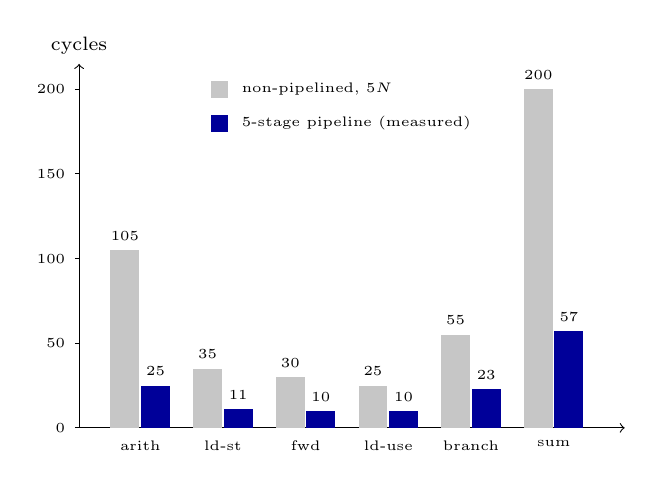
\begin{tikzpicture}[x=1.05cm, y=0.0215cm, font=\scriptsize]
\draw[->] (0,0) -- (6.6,0);
\draw[->] (0,0) -- (0,215) node[above, font=\scriptsize] {cycles};
\foreach \v in {0,50,100,150,200} {\draw (-0.05,\v) -- (0,\v); \node[anchor=east, font=\tiny] at (-0.05,\v) {\v};}
\foreach \i/\n/\c/\name in {1/21/25/arith, 2/7/11/ld-st, 3/6/10/fwd, 4/5/10/ld-use, 5/11/23/branch, 6/40/57/sum} {
  \pgfmathtruncatemacro{\b}{5*\n}
  \fill[gray!45] (\i-0.62,0) rectangle (\i-0.27,\b);
  \fill[blue!60!black] (\i-0.25,0) rectangle (\i+0.1,\c);
  \node[font=\tiny, anchor=south] at (\i-0.445,\b) {\b};
  \node[font=\tiny, anchor=south] at (\i-0.075,\c) {\c};
  \node[font=\tiny, anchor=north] at (\i-0.26,-2) {\name};
}
\fill[gray!45] (1.6,195) rectangle (1.8,205); \node[anchor=west, font=\tiny] at (1.85,200) {non-pipelined, $5N$};
\fill[blue!60!black] (1.6,175) rectangle (1.8,185); \node[anchor=west, font=\tiny] at (1.85,180) {5-stage pipeline (measured)};
\end{tikzpicture}
\caption{Total cycles per test program: measured five-stage pipeline versus a
non-pipelined baseline that needs five cycles per instruction at the same clock period.}
\label{fig:cycles}
\end{figure}

\subsection*{Demonstration Video}
A demonstration video introducing the team, the design and the simulation results is
available at \url{https://drive.google.com/drive/folders/1MsBRF6YmyPTbTrJbZ43O3noa1C6fjQQy?usp=sharing}.

\subsection*{Limitations and Phase II Plan}
The design supports only word loads and stores, a subset of branches, and no CSR,
exception or interrupt handling. Branches use static not-taken prediction, so every taken
branch costs two cycles. The hazard unit also compares the \texttt{rs2} field for every
instruction, so an I-type instruction whose immediate bits happen to match a load's
destination can stall one unnecessary cycle; this is safe but slightly conservative.
Phase~II will add synthesis results, larger benchmark programs and a fuller performance
discussion.

% ---------------------------------------------------------------------------

\subsection{Phase II Verification Coverage}
\label{sec:phase2-verification}
The Phase II regression command is
\texttt{bash simulation/run\_all.sh}. It combines 17 unit testbenches,
six Phase I programs on the pipeline, six Phase I programs on the single-cycle
baseline, twelve benchmark/design runs, and twelve differential
pipeline/baseline programs. The benchmark runner prints one
\texttt{BENCH} line per run and the equivalence runner prints one
\texttt{EQUIV} line per program. The raw benchmark and synthesis values used
by this report are stored in \texttt{analysis/results/perf.csv},
\texttt{analysis/results/speedup.csv}, and \texttt{synth/reports/summary.csv}.

\begin{table}[!t]
\centering
\caption{Phase II Regression Suites}
\label{tab:phase2-tests}
\begin{tabular}{@{}lrl@{}}
\toprule
\textbf{Suite} & \textbf{Runs} & \textbf{Coverage} \\
\midrule
Unit testbenches & 17 & Module-level directed and self-checking tests \\
Phase I pipeline & 6 & Architectural state on \texttt{riscv\_pipeline\_top} \\
Phase I baseline & 6 & Architectural state on \texttt{riscv\_single\_cycle\_top} \\
Benchmarks & 12 & Six programs on both designs \\
Equivalence & 12 & Six Phase I programs and six benchmarks \\
\bottomrule
\end{tabular}
\end{table}
